\subsection{بخش ب}
در این بخش به بررسی عملکرد هدایت تناسبی خالص برای مقادیر مختلف N پرداخته شده است. نتایج فرمان هدایت و نرخ چرخش در ادامه آمده است.

\begin{figure}[H]
	\centering
	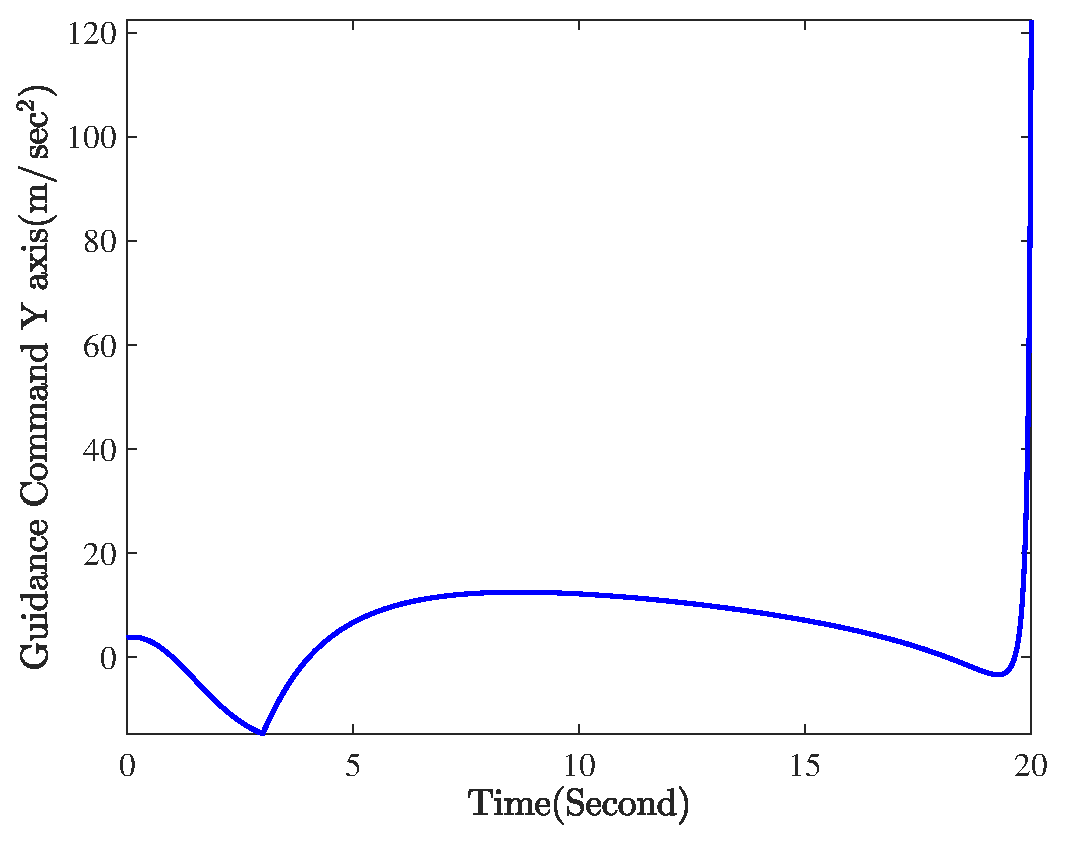
\includegraphics[width=.75\linewidth]{../Figure/Q1/b/GC_y_3}
	\caption{فرمان هدایت تناسبی در جهت محور
		 \lr{y}
	 برای 
	 $N=3$}
\end{figure}

\begin{figure}[H]
	\centering
	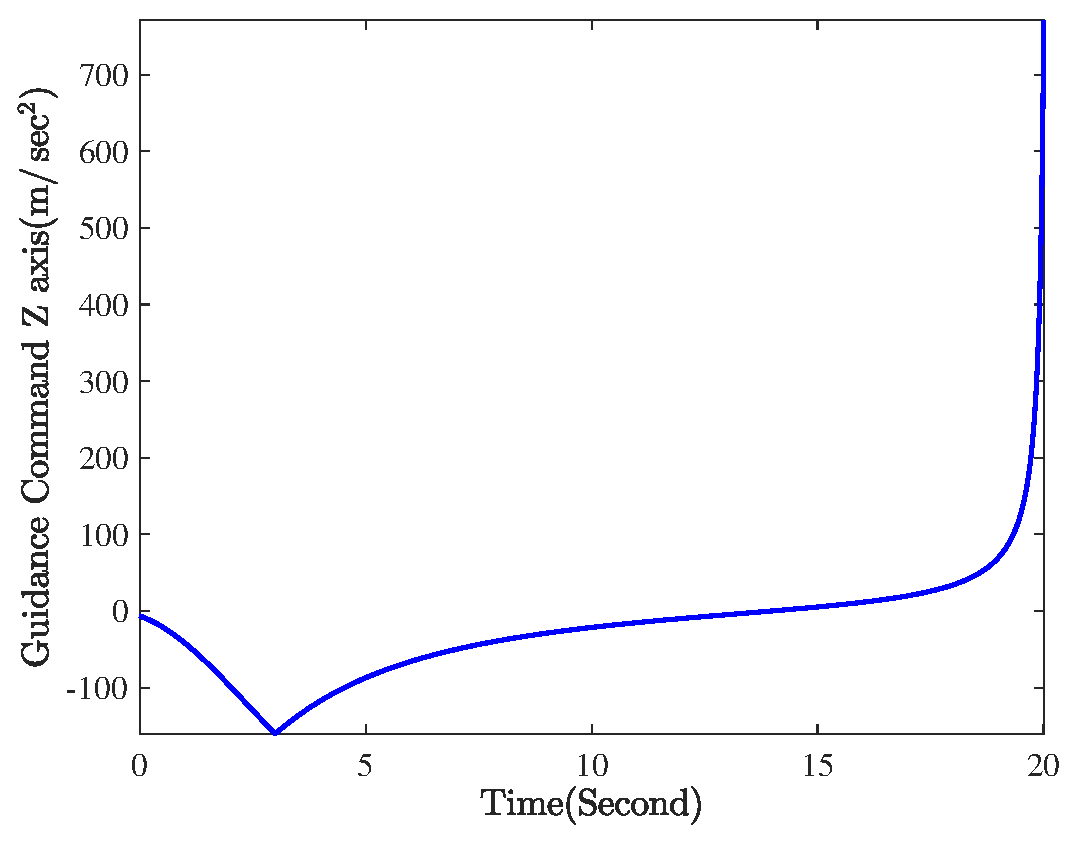
\includegraphics[width=.75\linewidth]{../Figure/Q1/b/GC_z_3}
	\caption{فرمان هدایت تناسبی در جهت محور
		\lr{z}
		برای 
		$N=3$}
\end{figure}

\begin{figure}[H]
	\centering
	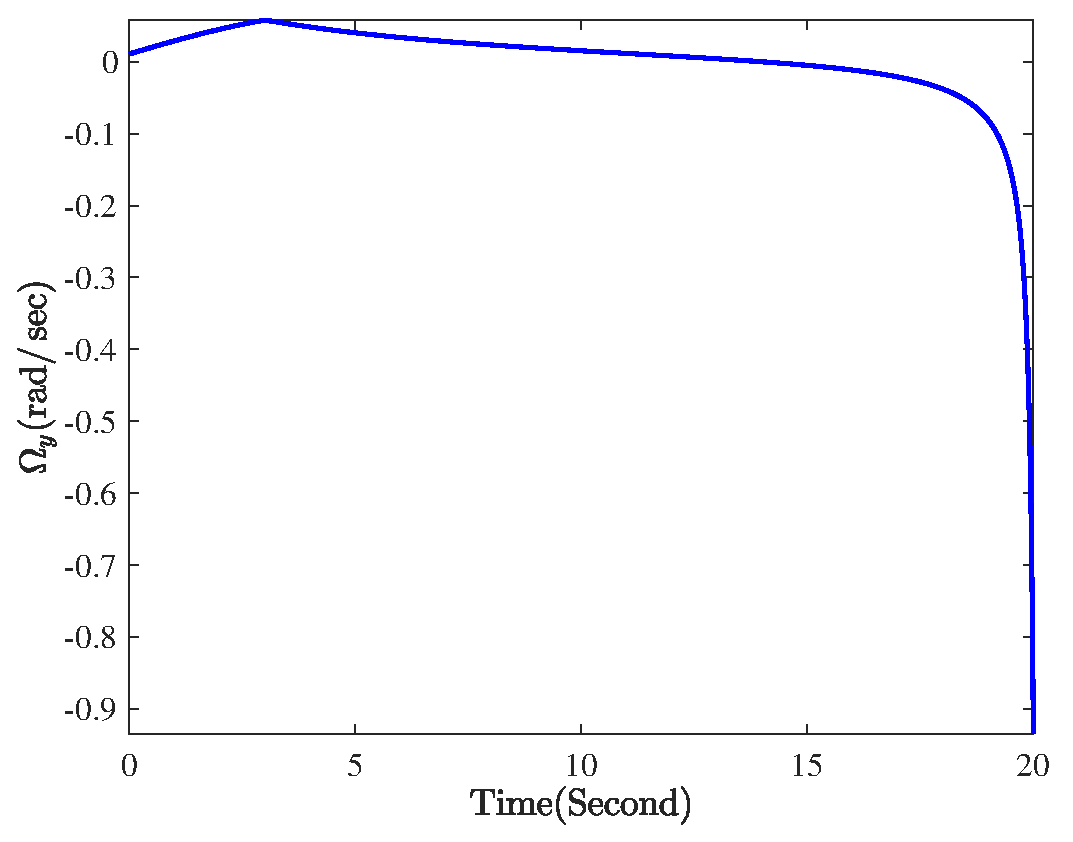
\includegraphics[width=.75\linewidth]{../Figure/Q1/b/Omega_y_3}
	\caption{ نرخ چرخش حول محور
		\lr{y}
		برای 
		$N=3$}
\end{figure}

\begin{figure}[H]
	\centering
	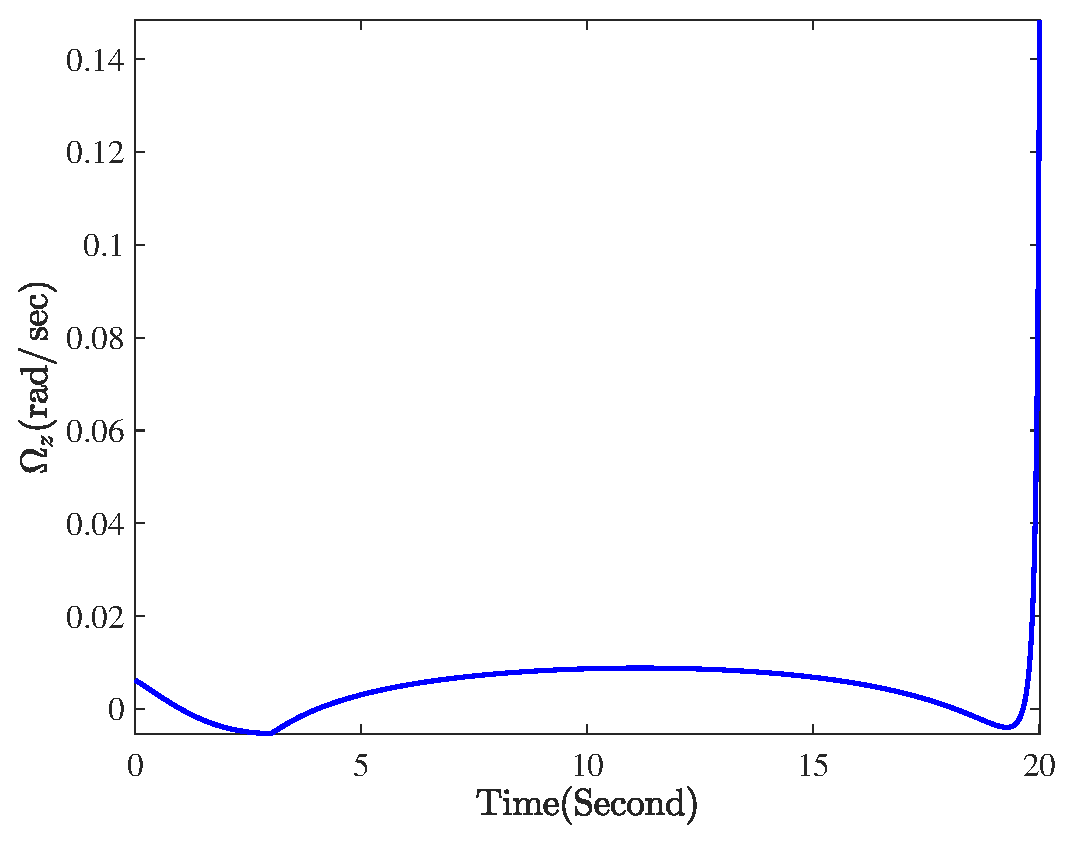
\includegraphics[width=.75\linewidth]{../Figure/Q1/b/Omega_z_3}
	\caption{ نرخ چرخش حول محور
		\lr{z}
		برای 
		$N=3$}
\end{figure}

%%%%%%%%%%%%%%%%%%%%%%%%%%%

\begin{figure}[H]
	\centering
	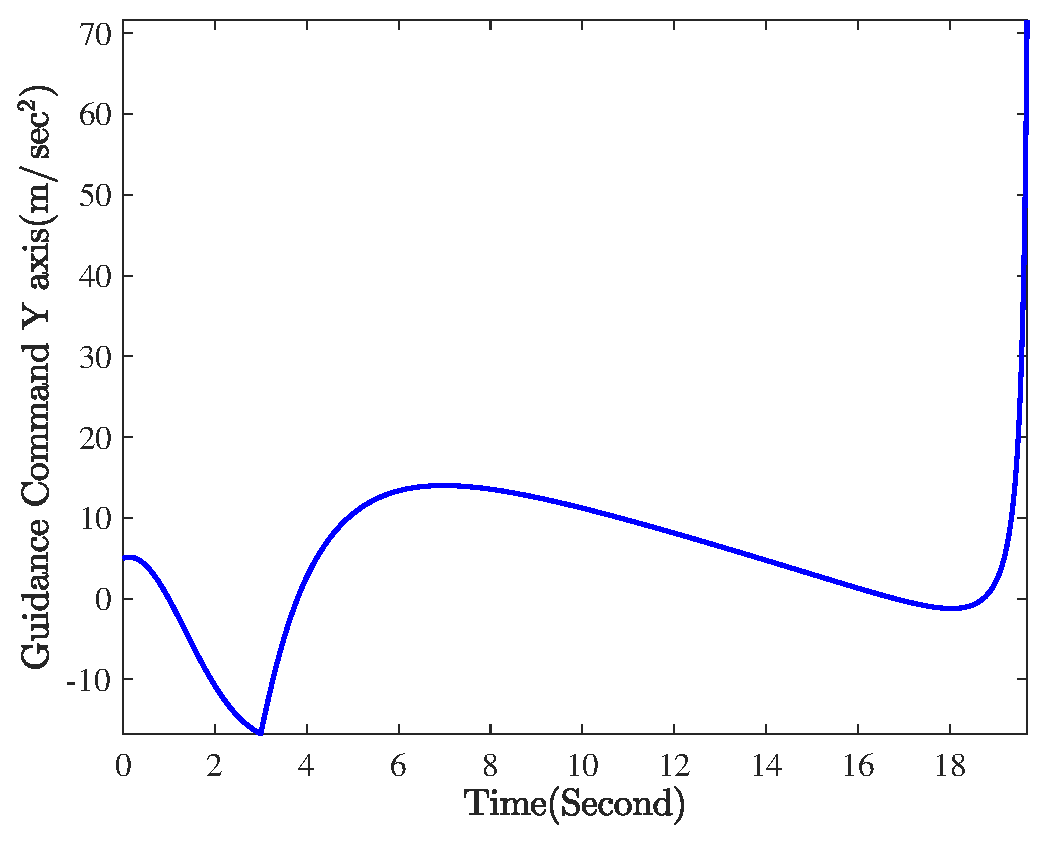
\includegraphics[width=.75\linewidth]{../Figure/Q1/b/GC_y_4}
	\caption{فرمان هدایت تناسبی در جهت محور
		\lr{y}
		برای 
		$N=4$}
\end{figure}

\begin{figure}[H]
	\centering
	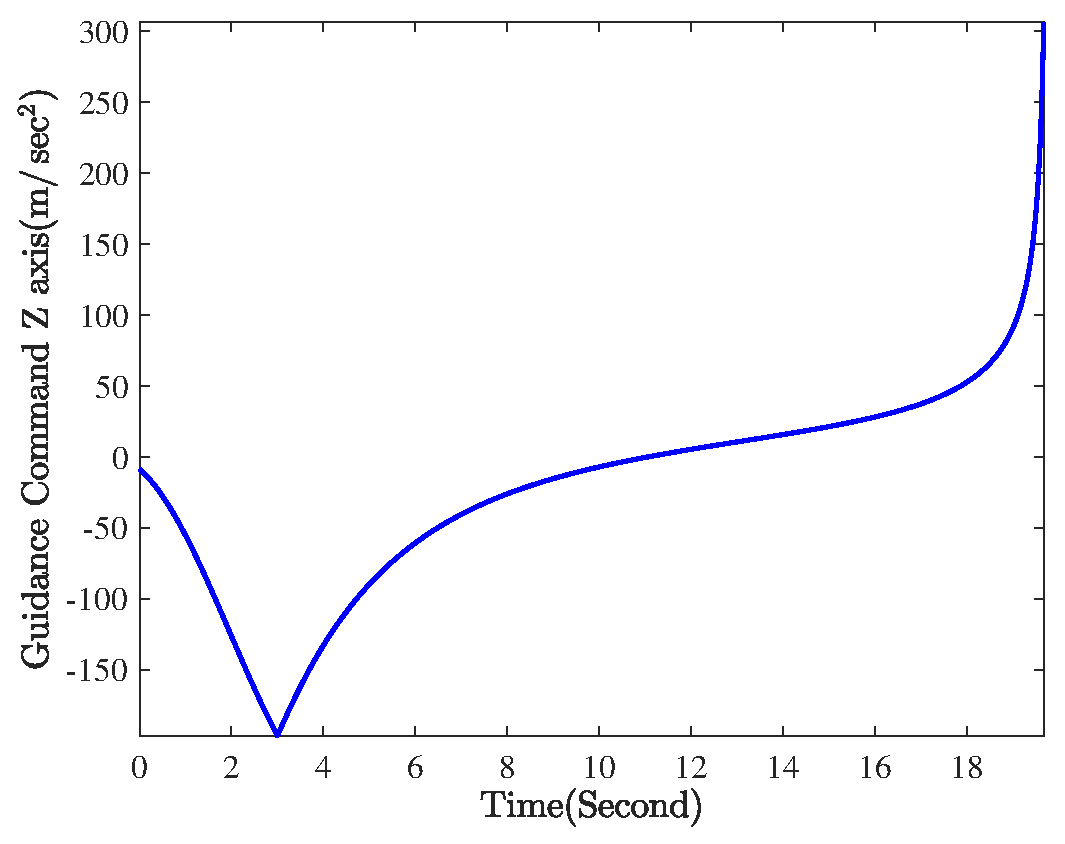
\includegraphics[width=.75\linewidth]{../Figure/Q1/b/GC_z_4}
	\caption{فرمان هدایت تناسبی در جهت محور
		\lr{z}
		برای 
		$N=4$}
\end{figure}

\begin{figure}[H]
	\centering
	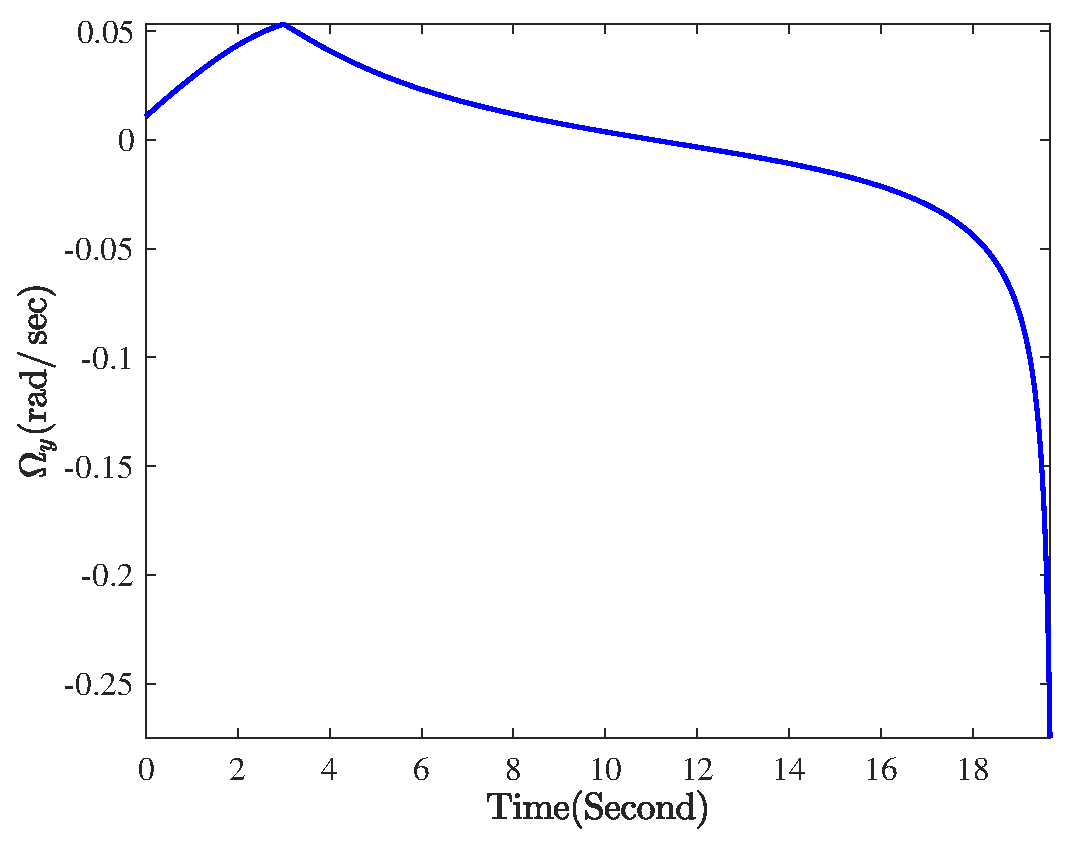
\includegraphics[width=.75\linewidth]{../Figure/Q1/b/Omega_y_4}
	\caption{ نرخ چرخش حول محور
		\lr{y}
		برای 
		$N=4$}
\end{figure}

\begin{figure}[H]
	\centering
	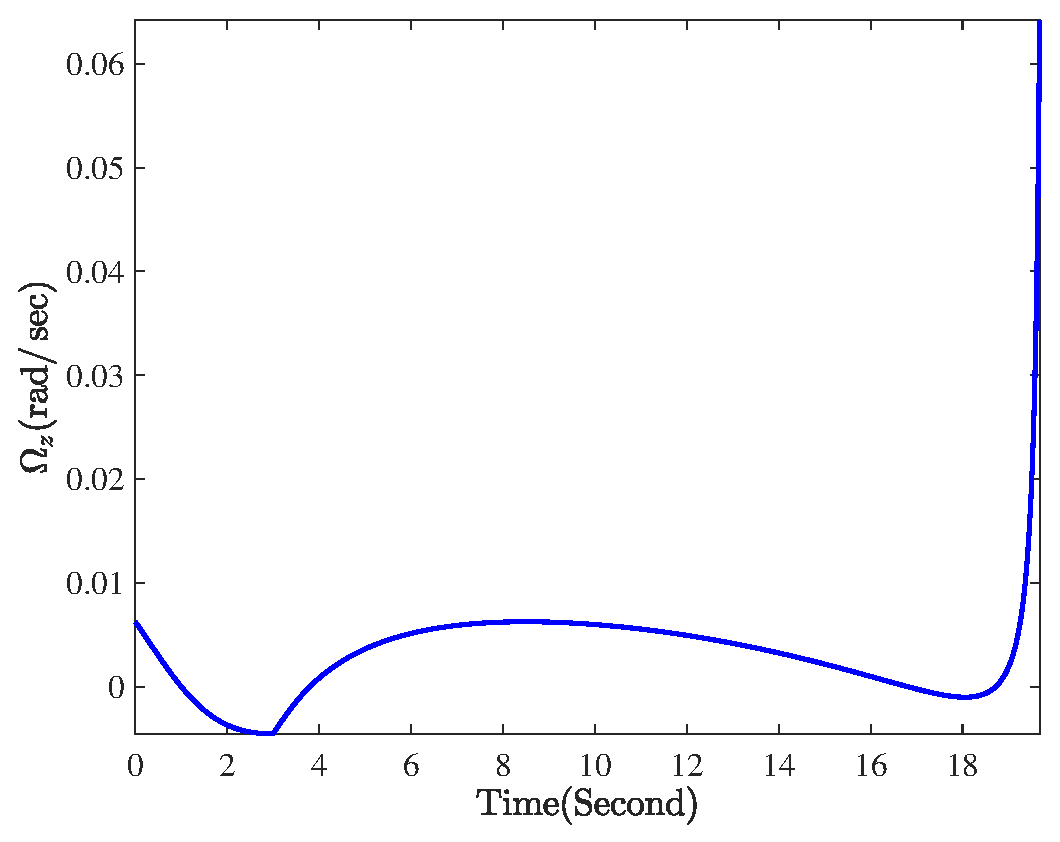
\includegraphics[width=.75\linewidth]{../Figure/Q1/b/Omega_z_4}
	\caption{ نرخ چرخش حول محور
		\lr{z}
		برای 
		$N=4$}
\end{figure}
%%%%%%%%%%%%%%%%%%%%%
\begin{figure}[H]
	\centering
	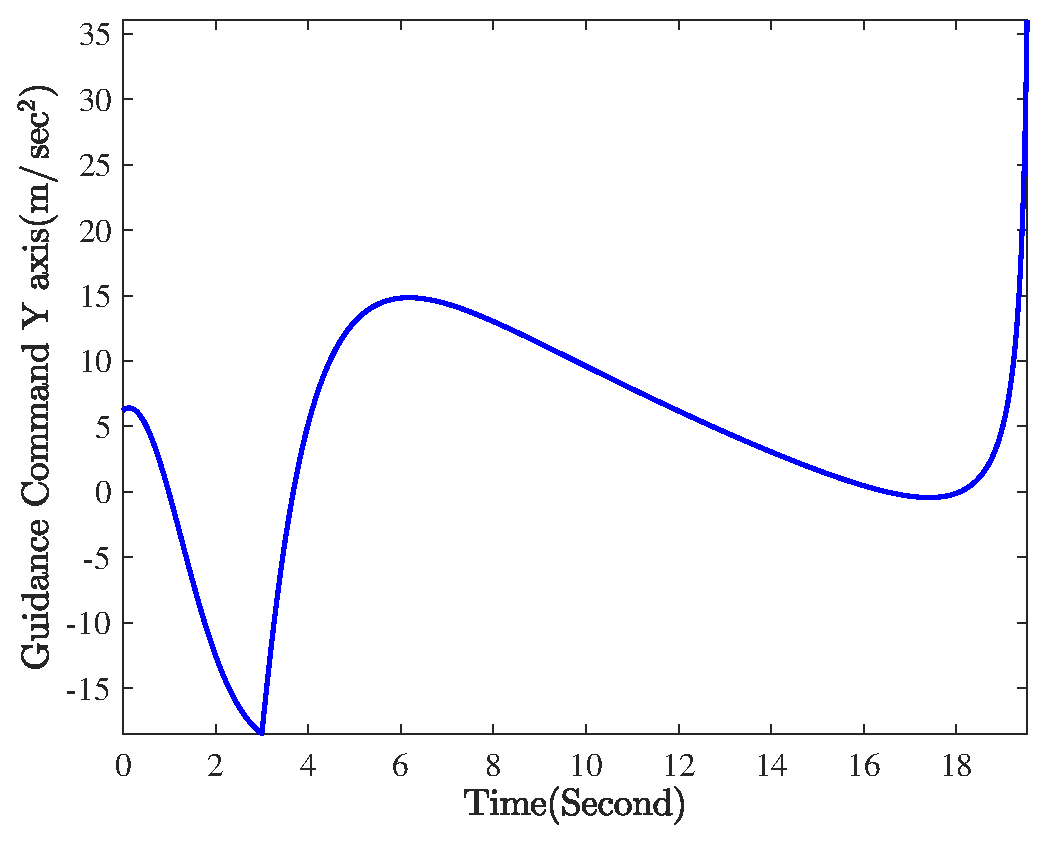
\includegraphics[width=.75\linewidth]{../Figure/Q1/b/GC_y_5}
	\caption{فرمان هدایت تناسبی در جهت محور
		\lr{y}
		برای 
		$N=5$}
\end{figure}

\begin{figure}[H]
	\centering
	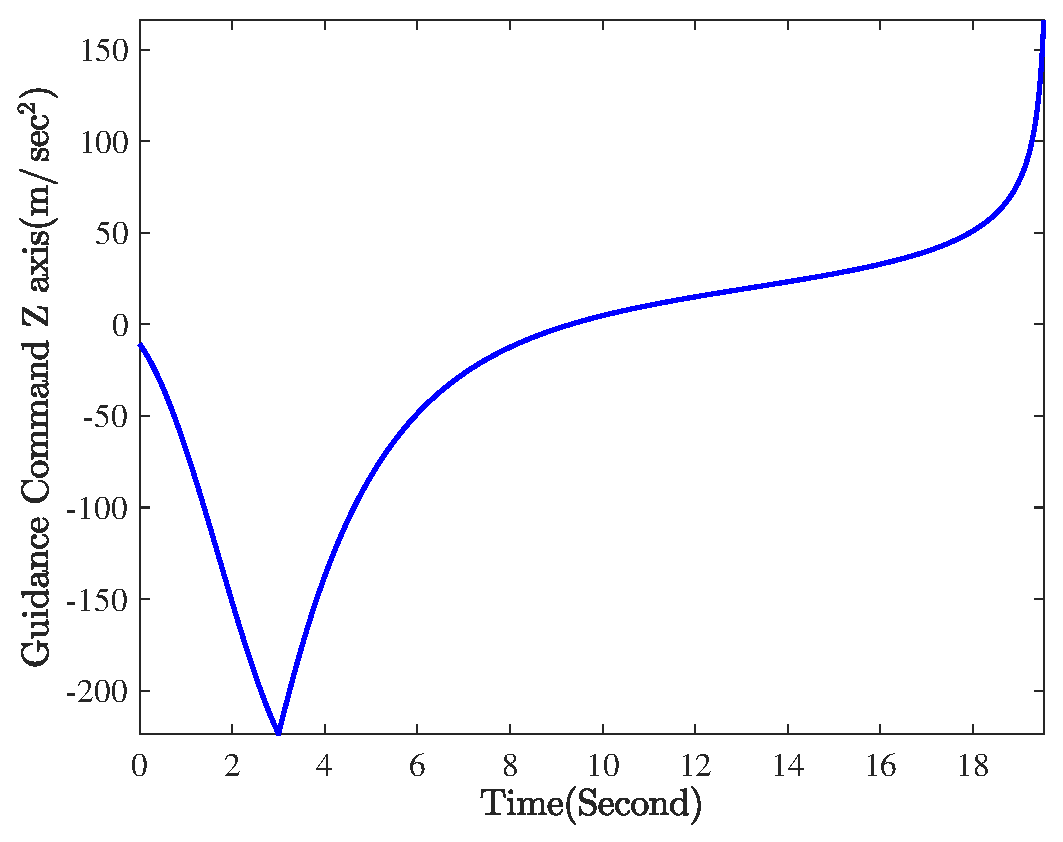
\includegraphics[width=.75\linewidth]{../Figure/Q1/b/GC_z_5}
	\caption{فرمان هدایت تناسبی در جهت محور
		\lr{z}
		برای 
		$N=5$}
\end{figure}

\begin{figure}[H]
	\centering
	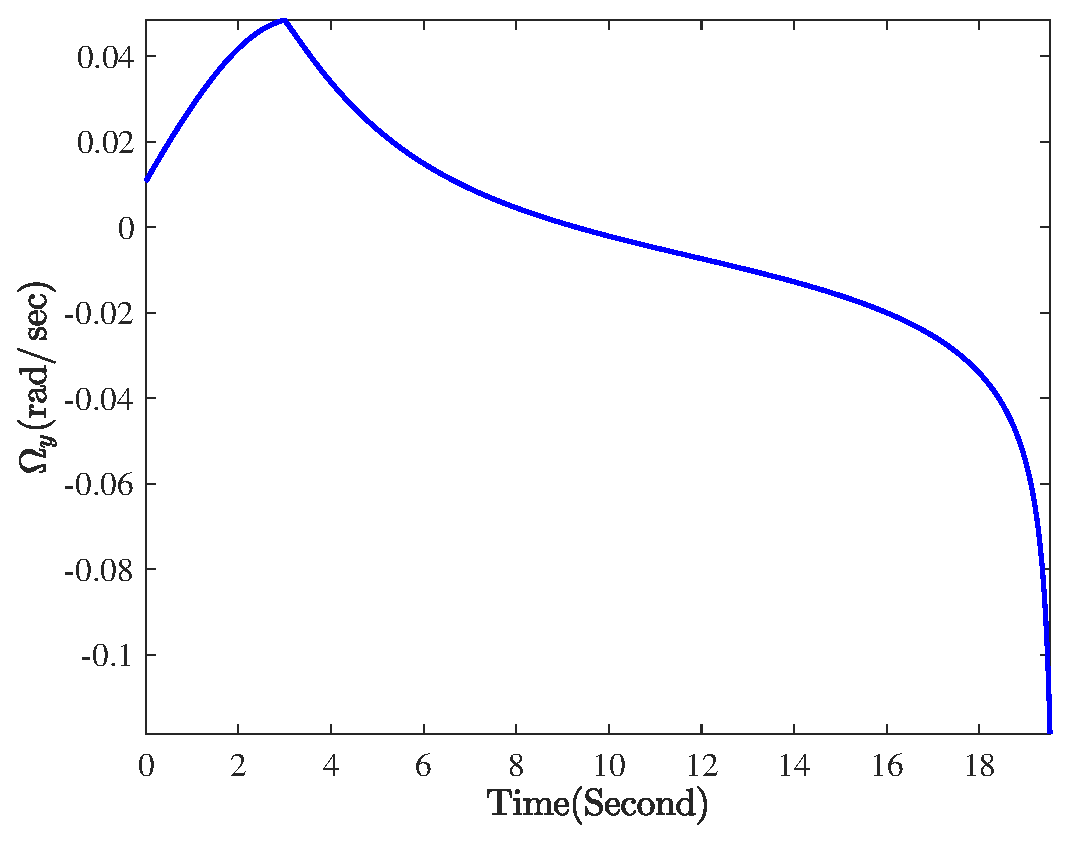
\includegraphics[width=.75\linewidth]{../Figure/Q1/b/Omega_y_5}
	\caption{ نرخ چرخش حول محور
		\lr{y}
		برای 
		$N=5$}
\end{figure}

\begin{figure}[H]
	\centering
	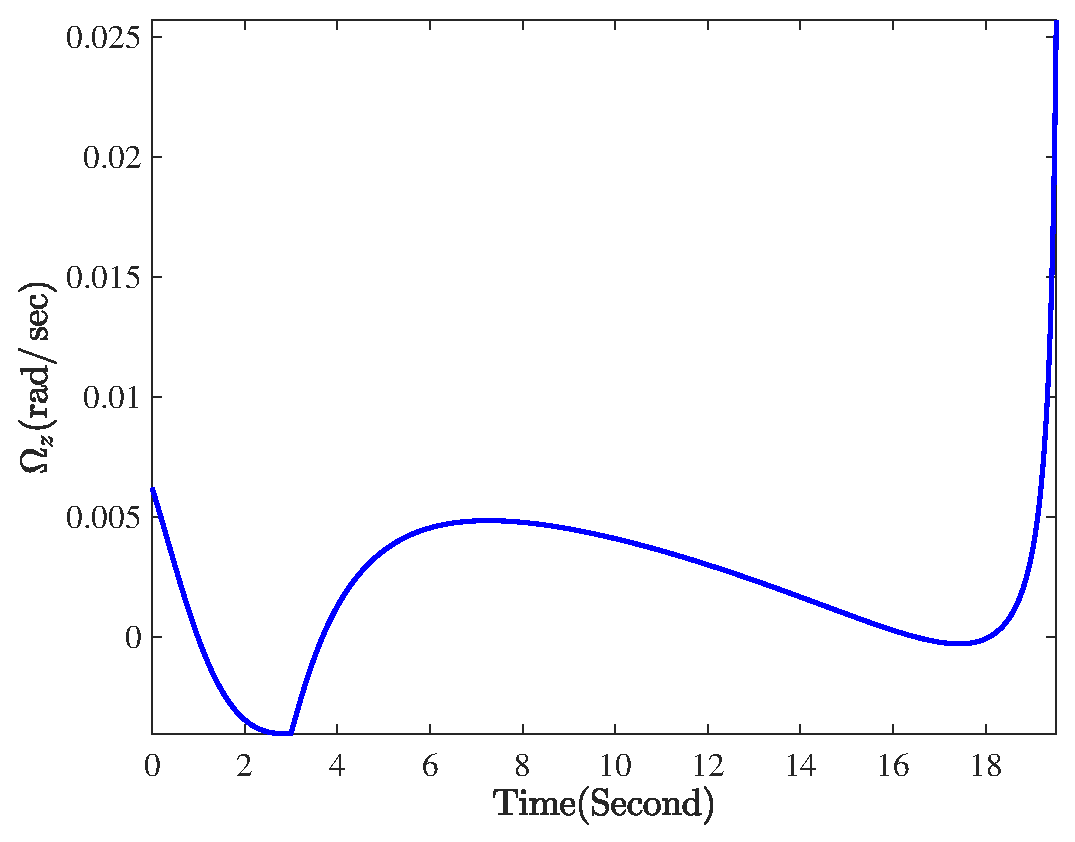
\includegraphics[width=.75\linewidth]{../Figure/Q1/b/Omega_z_5}
	\caption{ نرخ چرخش حول محور
		\lr{z}
		برای 
		$N=5$}
\end{figure}


%%%%%%%%%%%%%%%%%%%%%
\begin{figure}[H]
	\centering
	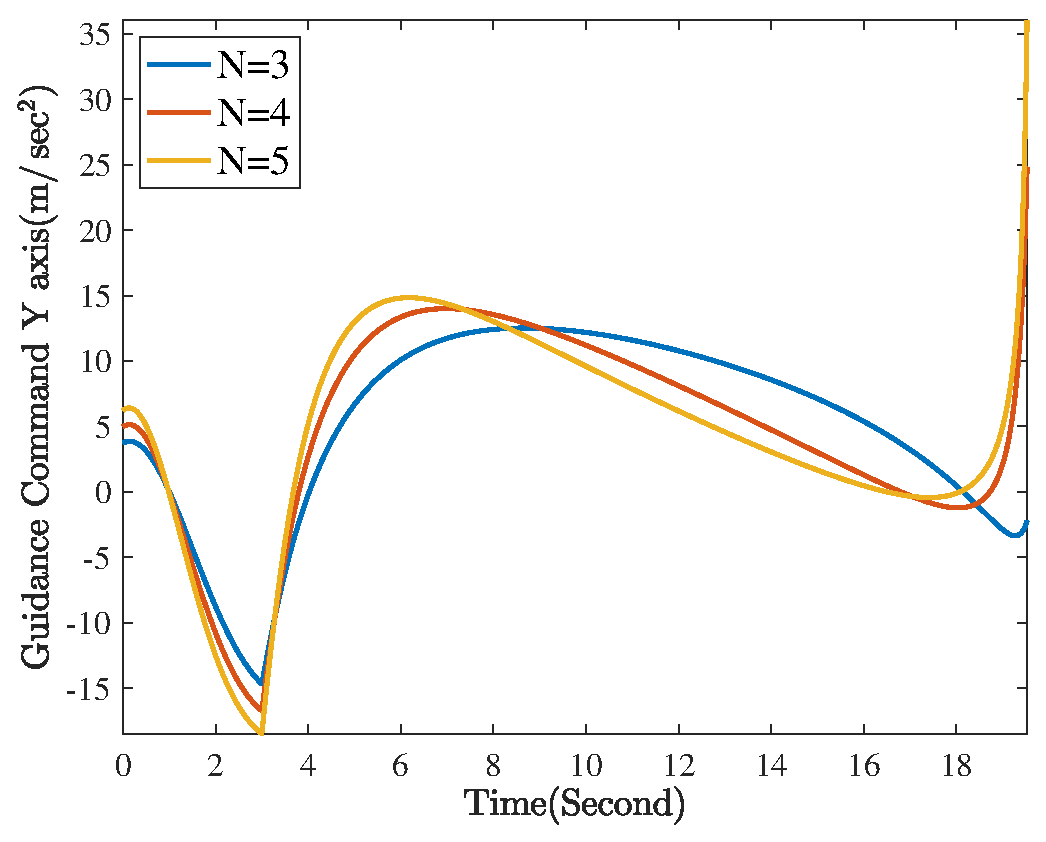
\includegraphics[width=.75\linewidth]{../Figure/Q1/b/GC_y}
	\caption{فرمان هدایت تناسبی در جهت محور
		\lr{y}
		برای 
		تمامی مقادیر N}
\end{figure}

\begin{figure}[H]
	\centering
	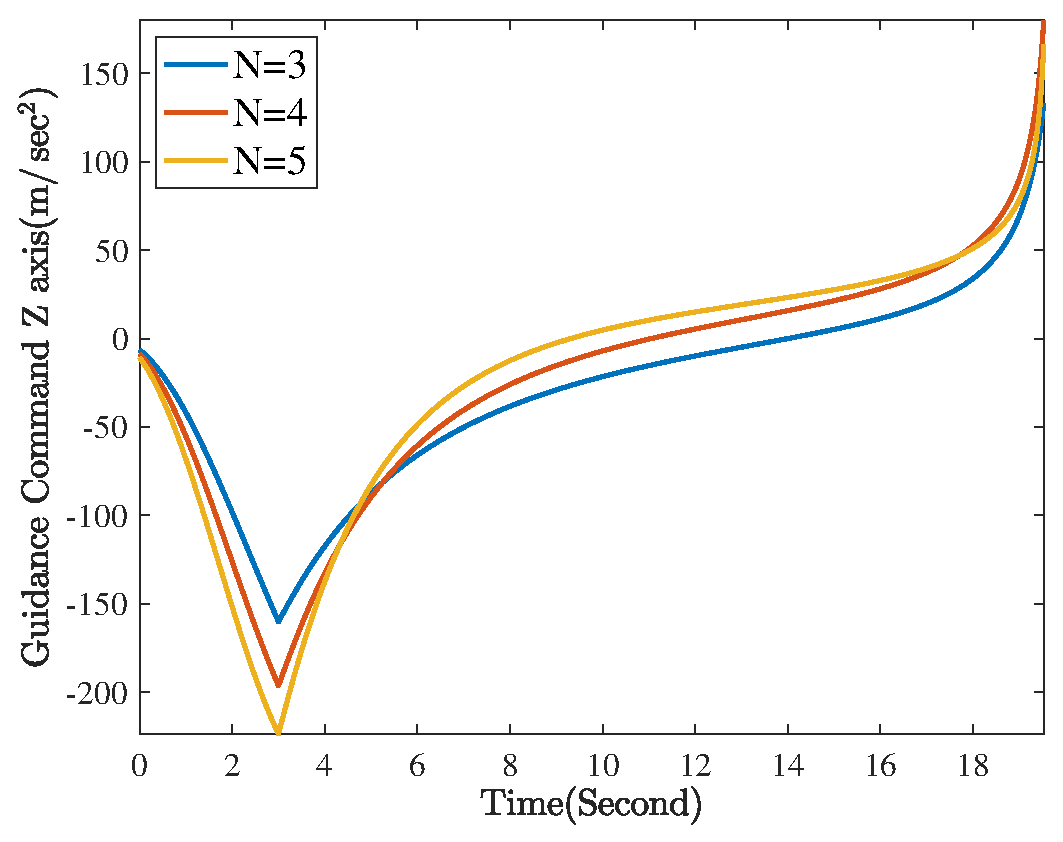
\includegraphics[width=.75\linewidth]{../Figure/Q1/b/GC_z}
	\caption{فرمان هدایت تناسبی در جهت محور
		\lr{z}
		برای 
		تمامی مقادیر N}
\end{figure}

\begin{figure}[H]
	\centering
	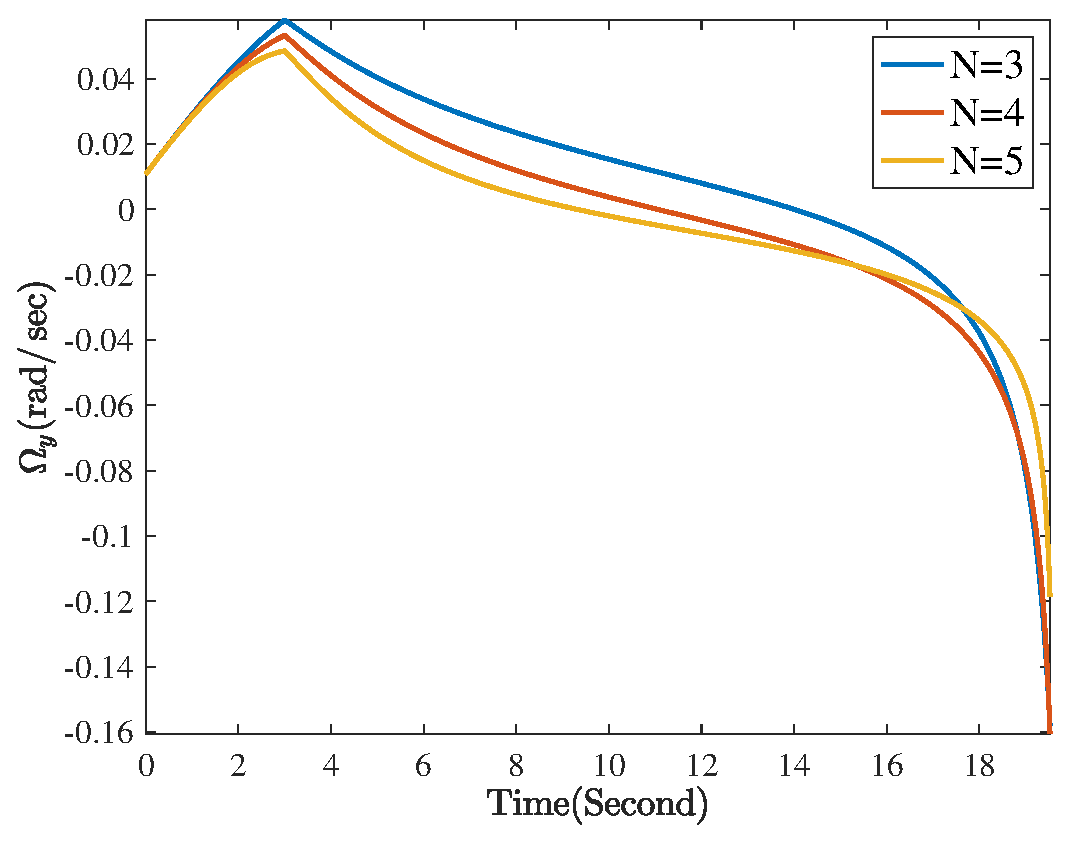
\includegraphics[width=.75\linewidth]{../Figure/Q1/b/Omega_y}
	\caption{ نرخ چرخش حول محور
		\lr{y}
		برای 
		تمامی مقادیر N}
\end{figure}

\begin{figure}[H]
	\centering
	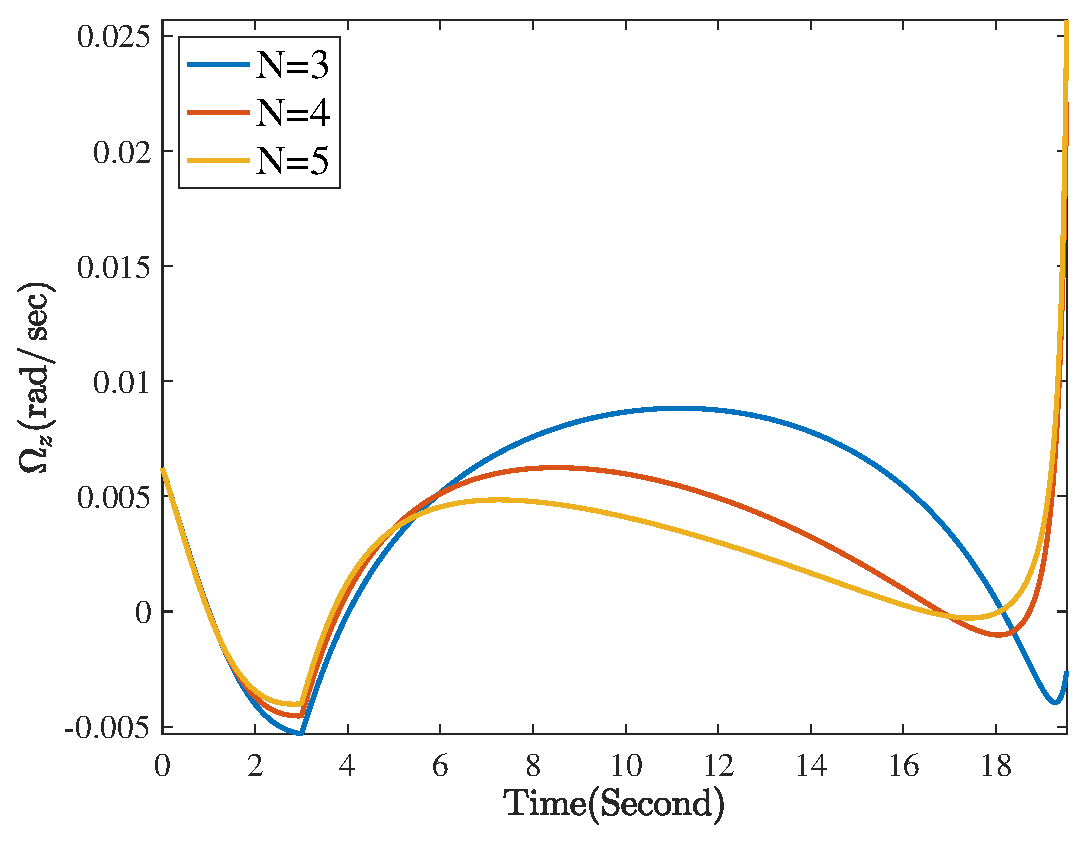
\includegraphics[width=.75\linewidth]{../Figure/Q1/b/Omega_z}
	\caption{ نرخ چرخش حول محور
		\lr{z}
		برای 
		تمامی مقادیر N}
\end{figure}



بر اساس نمودارهای فرمان شتاب، ضریب هدایت بیشتر فرمان شتاب هدایت بیشتری تولید می‌کند. بنابراین نرخ چرخش خط دید ستریع‌تر کاهش می‌یابد و به صفر می‌رسد. به همین دلیل، در انتهای ماموریت دستور شتاب کمتری دارد و باعث می‌شود وارد محدوده اشباع نشود. در انتهای ماموریت $t= t_f$ تکینگی وجود دارد که در نمودارها دیده می‌شود. در بخش‌های آینده با استفاده از فرمان‌های قبلی در نزدیکی هدف، این مشکل برطرف شده است.